\documentclass[twocolumn]{aastex63}

% typography
\usepackage[T1]{fontenc}

\setlength{\parindent}{1.\baselineskip}
\newcommand{\acronym}[1]{{\small{#1}}}
\newcommand{\package}[1]{\textsl{#1}}
\newcommand{\gaia}{\textsl{Gaia}}
% \newcommand{\hst}{\textsl{HST}}
% \newcommand{\pans}{\textsl{Pan-STARRS}}

% \newcommand{\deg}{\ensuremath{\textrm{deg}}}
\newcommand{\msun}{\ensuremath{\textrm{M}_\odot}}
\newcommand{\myr}{\ensuremath{\textrm{Myr}}}
\newcommand{\gyr}{\ensuremath{\textrm{Gyr}}}
\newcommand{\kpc}{\ensuremath{\textrm{kpc}}}
\newcommand{\kms}{\ensuremath{\textrm{km}\,\textrm{s}^{-1}}}
\newcommand{\masyr}{\ensuremath{\textrm{mas}\,\textrm{yr}^{-1}}}
\newcommand{\feh}{\ensuremath{\textrm{[Fe/H]}}}
\newcommand{\afe}{\ensuremath{\textrm{[$\alpha$/Fe]}}}
\newcommand{\changes}[1]{{\textbf{#1}}}
\hyphenation{kruijs-sen}

% aastex parameters
% \received{not yet; THIS IS A DRAFT}
%\revised{not yet}
%\accepted{not yet}
% % Adds "Submitted to " the argument.
% \submitjournal{ApJ}
\shorttitle{}
\shortauthors{bonaca \& kruijssen}

%@arxiver{}
\usepackage{amsmath}

\begin{document}\sloppy\sloppypar\raggedbottom\frenchspacing % trust me

\title{The low masses of globular clusters that dissolved in the Milky Way}

\correspondingauthor{Ana~Bonaca}
\email{ana.bonaca@cfa.harvard.edu}

\author[0000-0002-7846-9787]{Ana~Bonaca}
\affil{Center for Astrophysics | Harvard \& Smithsonian, 60 Garden Street, Cambridge, MA 02138, USA}

\author[0000-0002-8804-0212]{J.~M.~Diederik~Kruijssen}
\affiliation{Astronomisches Rechen-Institut, Zentrum f\" ur Astronomie der Universit\" at Heidelberg, M\" onchhofstra\ss e 12-14, D-69120 Heidelberg, Germany}
\affil{Center for Astrophysics | Harvard \& Smithsonian, 60 Garden Street, Cambridge, MA 02138, USA}


\begin{abstract}\noindent % trust me
Numerous stellar streams that have been discovered in the Milky Way as evaporated globular clusters show signs of dynamical perturbation.
N-body models that can illuminate the origin of these perturbations require the cluster's initial mass as a fundamental input parameter.
Here we present orbits and masses of 20 dissolved globular clusters in the Milky Way.
We constrained the streams' orbits by fitting the 3D positions of a stream's endpoints from ground-based photometry and its proper motions from Gaia.
Assuming a dissolution time of 10\,Gyr, we use orbital apocenters and eccentricities to estimate the clusters' initial mass.
Disrupted globular clusters have preferentially lower masses than the surviving population, with the median mass being an order of magnitude smaller.
The overall distribution of apocenters and eccentricities is similar for the disrupted and surviving clusters, however, at a fixed mass disrupted clusters have smaller apocenters and larger eccentricities.
The progenitors of tidal streams observed at the present are a specific, low-mass subset of the initial globular cluster population.
This has implications for establishing the role of internal dynamics in sculpting the observed tidal debris, and the amount of external perturbation, e.g., from dark-matter subhalos, that these streams experienced.
\end{abstract}

\section{Introduction}
\label{sec:intro}

Theoretical studies of globular cluster dynamics predicted that stars escape globular clusters due to two-body relaxation and tidal stripping \citep[e.g.,][]{spitzer:1987, baumgardt03}, forming long and thin tidal tails along the cluster's orbit \citep{combes:1999}.
Such tidal tails were first detected around the Palomar~5 globular cluster \citep{odenkirchen:2001, rockosi:2002}.
Stellar streams of similar width and length, but without a surviving progenitor, have been discovered throughout the Milky Way \citep[e.g.,][]{gd:2006, grillmair:2009, bonaca:2012, shipp:2018, ibata:2019}, likely constituting a population of completely dissolved globular clusters.

Forming kinematically cold and being shaped by the Milky Way tides, we expect that globular cluster streams are sensitive both to the global distribution of matter in the Galaxy \citep[e.g.,][]{lux:2013, bonaca:2014, sanders:2014}, and to small-scale perturbations, such as predicted from low-mass dark-matter subhalos \citep[e.g.,][]{ibata:2002, yoon:2011, erkal:2016}.
Detailed observations have recently revealed signatures of perturbation in a number of thin streams \citep[e.g.,][]{pwb, bonaca:2019a, bonaca:2020, li:2020}, which may be attributed to impacts of dark-matter subhalos \citep[e.g.,][]{bonaca:2019b, banik:2019}.
Alternatively, the observed features may be due to the way stars escape globular clusters \citep[e.g.,][]{kuepper:2008, kuepper:2010} or due to the onset of cluster disruption before its original host galaxy accreted onto the Milky Way \citep[e.g.,][]{carlberg:2018, malhan:2020}.

To employ tidal tails as cosmological tracers of dark matter, it is essential to disentangle the internal and external sources of perturbation.
Direct N-body simulations of the progenitor globular clusters in realistic environments would accurately capture the relevant processes \citep[e.g.,][]{renaud:2015}.
However, these simulations remain out of reach because a cluster's dynamical evolution sensitively depends on its mass \citep[e.g.,][]{hh:2003, balbinot:2018}, and masses of most dissolved clusters are extremely uncertain \citep[e.g.,][]{erkal:2016b}.

Our goal in this Letter is to dynamically estimate masses of disrupted globular clusters that are now observed as stellar streams in the Milky Way.
The timescale for cluster disruption is determined by its initial mass (more massive clusters take longer) and its orbit: clusters on more eccentric orbits and with smaller apocenters dissolve faster \citep{kruijssen09}.
Using data from the Gaia mission \citep{gdr2}, we determine stream orbits in Section~\ref{sec:orbits}.
Since the streams are coherent, we assume the progenitor globular clusters disrupted recently \citep{helmi:2003}, and in Section~\ref{sec:disrupted} calculate their masses.
We close by discussing the implications of the inferred low masses for dynamical studies of stellar streams, and place this population of disrupted globular clusters in the context of cluster and galaxy formation.

\begin{figure*}
\begin{center}
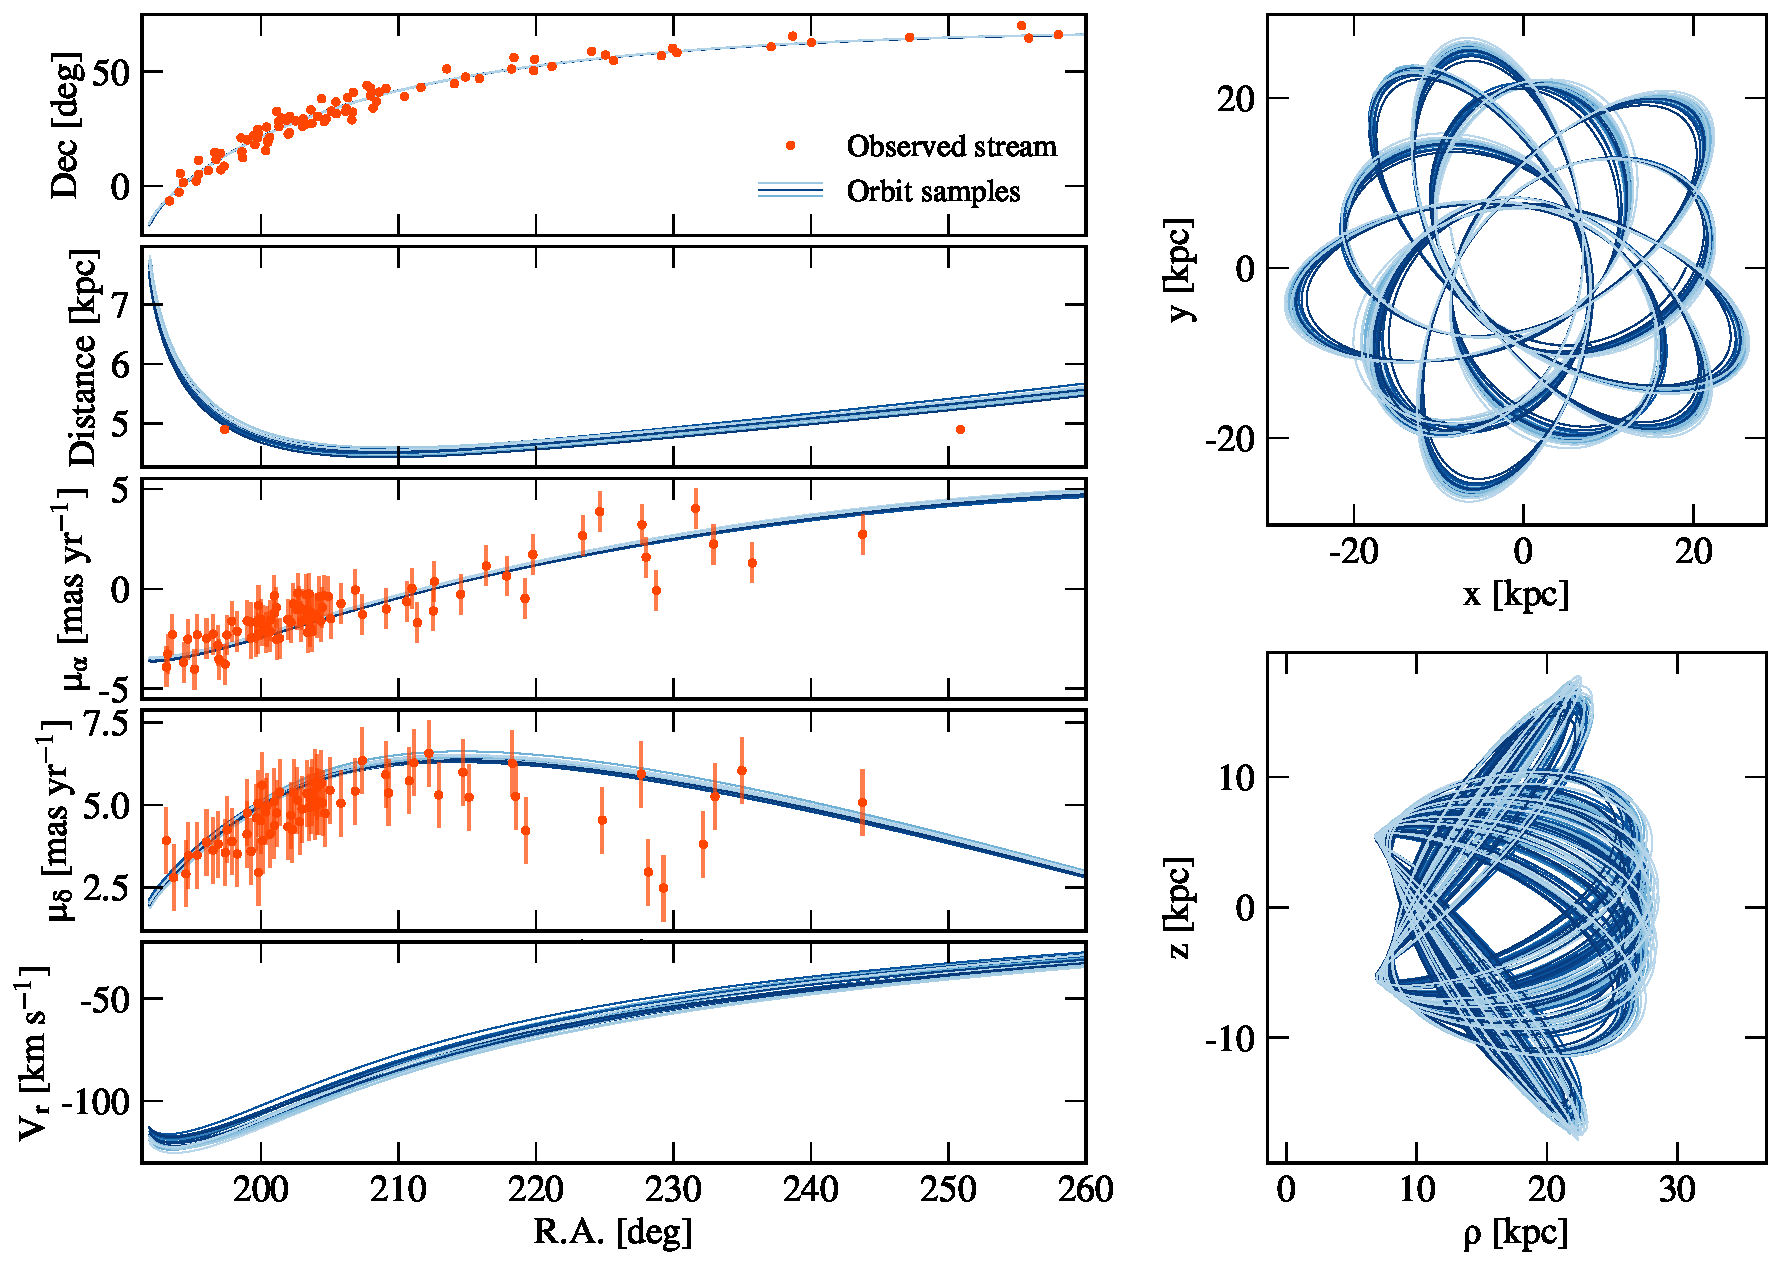
\includegraphics[width=0.9\textwidth]{figures/stream_fitting.pdf}
\end{center}
\caption{Orbital constraints for the Fj\"{o}rm stellar stream in the observed coordinates (left: panels from top to bottom show declination, distance, and proper motion components as a function of right ascension) and cylindrical Galactocentric coordinates (right: in and out of the Galactic plane for the top and bottom panels, respectively).
Different shades of blue represent orbit samples from the posterior constrained by the stream endpoints (orange points).
Current observations allow for a range of orbital apocenters and eccentricities.
}
\label{fig:streams}
\end{figure*}

\begin{deluxetable*}{l @{\hspace{0.5cm}} D D D D D D @{\hspace{0.8cm}} D D D}
\tablehead{
Name & \multicolumn2c{R.A.} & \multicolumn2c{Dec} & \multicolumn2c{d} & \multicolumn2c{$\mu_\alpha$} & \multicolumn2c{$\mu_\delta$} & \multicolumn2c{$V_r$} & \multicolumn2c{$r_{peri}$} & \multicolumn2c{$r_{apo}$} & \multicolumn2c{$\log M_i/\rm\msun$}\\
& \multicolumn2c{deg} & \multicolumn2c{deg} & \multicolumn2c{kpc} & \multicolumn2c{mas/yr} & \multicolumn2c{mas/yr} & \multicolumn2c{km/s} & \multicolumn2c{kpc} & \multicolumn2c{kpc} & \multicolumn2c{dex}
}
\decimals
\setlength{\tabcolsep}{3pt}
\startdata
ATLAS & $30.7$ & -33.2$^{+0.2}_{-0.2}$ & 21.7$^{+3.0}_{-3.0}$ & -0.1$^{+0.5}_{-0.5}$ & -0.7$^{+0.2}_{-0.2}$ & 96.7$^{+87.7}_{-96.9}$ & 17.7$^{+5.0}_{-5.2}$ & 32.3$^{+22.7}_{-7.0}$ & $3.61\pm0.19$ \\ 
Aliqa Uma & $40.6$ & -38.3$^{+0.2}_{-0.2}$ & 27.6$^{+3.6}_{-3.7}$ & 0.2$^{+0.4}_{-0.4}$ & -0.2$^{+0.3}_{-0.3}$ & 147.8$^{+155.2}_{-173.4}$ & 17.8$^{+8.5}_{-5.9}$ & 48.3$^{+65.2}_{-15.6}$ & $3.49\pm0.25$ \\ 
Chenab & $-28.3$ & -43.0$^{+0.5}_{-0.5}$ & 39.1$^{+5.0}_{-4.8}$ & -0.1$^{+0.2}_{-0.2}$ & -2.5$^{+0.4}_{-0.5}$ & 27.0$^{+103.6}_{-111.5}$ & 28.6$^{+6.9}_{-11.4}$ & 63.9$^{+73.3}_{-26.2}$ & $3.23\pm0.32$ \\ 
Elqui & $20.6$ & -42.4$^{+0.3}_{-0.3}$ & 48.6$^{+6.2}_{-6.1}$ & -0.1$^{+0.3}_{-0.3}$ & -0.3$^{+0.2}_{-0.2}$ & 98.4$^{+160.2}_{-155.8}$ & 33.3$^{+12.8}_{-14.3}$ & 91.4$^{+98.8}_{-35.3}$ & $3.08\pm0.30$ \\ 
Fimbulthul & $214.2$ & -22.6$^{+0.3}_{-0.3}$ & 4.2$^{+0.0}_{-0.0}$ & -15.1$^{+0.3}_{-0.3}$ & -10.1$^{+0.4}_{-0.4}$ & 74.6$^{+1.9}_{-1.8}$ &  1.5$^{+0.1}_{-0.1}$ &  7.1$^{+0.1}_{-0.1}$ & $5.10\pm0.05$ \\ 
Fj\"{o}rm & $197.4$ & 5.6$^{+0.4}_{-0.4}$ & 4.9$^{+0.0}_{-0.1}$ & -3.7$^{+0.2}_{-0.3}$ & 3.9$^{+0.4}_{-0.4}$ & -113.0$^{+8.8}_{-8.5}$ &  8.2$^{+0.0}_{-0.0}$ & 24.0$^{+3.0}_{-2.9}$ & $4.03\pm0.03$ \\ 
Gj\"{o}ll & $70.2$ & -2.6$^{+0.3}_{-0.3}$ & 3.5$^{+0.1}_{-0.1}$ & 22.1$^{+0.5}_{-0.5}$ & -22.9$^{+0.5}_{-0.5}$ & -25.8$^{+11.8}_{-11.2}$ &  9.3$^{+0.2}_{-0.2}$ & 29.6$^{+3.6}_{-3.0}$ & $3.93\pm0.03$ \\ 
Indus & $-36.3$ & -50.7$^{+0.6}_{-0.6}$ & 16.5$^{+1.8}_{-1.6}$ & 2.6$^{+0.4}_{-0.3}$ & -5.9$^{+0.5}_{-0.6}$ & 4.4$^{+64.6}_{-71.6}$ & 11.7$^{+2.1}_{-3.1}$ & 28.2$^{+30.8}_{-11.6}$ & $3.85\pm0.23$ \\ 
Leiptr & $61.0$ & 0.7$^{+0.3}_{-0.3}$ & 8.3$^{+0.3}_{-0.2}$ & 8.9$^{+0.4}_{-0.4}$ & -10.1$^{+0.5}_{-0.5}$ & -84.0$^{+18.3}_{-18.8}$ & 12.8$^{+0.4}_{-0.4}$ & 45.4$^{+14.3}_{-10.8}$ & $3.68\pm0.07$ \\ 
Phoenix & $20.1$ & -55.3$^{+0.1}_{-0.1}$ & 18.5$^{+1.7}_{-1.4}$ & 2.8$^{+0.3}_{-0.3}$ & 0.3$^{+0.5}_{-0.4}$ & 115.6$^{+107.1}_{-118.6}$ & 12.1$^{+5.1}_{-4.5}$ & 26.3$^{+18.1}_{-6.1}$ & $3.84\pm0.20$ \\ 
Ravi & $-16.0$ & -59.6$^{+0.5}_{-0.5}$ & 21.7$^{+3.2}_{-3.0}$ & 0.6$^{+0.3}_{-0.2}$ & -1.0$^{+0.4}_{-0.3}$ & 148.3$^{+71.6}_{-81.7}$ &  7.1$^{+3.7}_{-2.6}$ & 21.2$^{+4.2}_{-2.9}$ & $4.12\pm0.20$ \\ 
Slidr & $178.0$ & 3.3$^{+0.4}_{-0.3}$ & 3.4$^{+0.1}_{-0.1}$ & -25.5$^{+0.6}_{-0.6}$ & -3.6$^{+0.3}_{-0.3}$ & 78.5$^{+9.1}_{-9.1}$ &  2.4$^{+0.3}_{-0.3}$ & 27.2$^{+2.1}_{-1.9}$ & $4.65\pm0.07$ \\ 
Sv\"{o}l & $244.4$ & 23.5$^{+0.3}_{-0.4}$ & 8.1$^{+0.1}_{-0.2}$ & -4.4$^{+0.1}_{-0.1}$ & -0.9$^{+0.2}_{-0.2}$ & -109.0$^{+4.8}_{-5.4}$ &  1.0$^{+0.1}_{-0.1}$ &  8.7$^{+0.1}_{-0.2}$ & $5.27\pm0.04$ \\ 
Sylgr & $186.6$ & -0.8$^{+0.3}_{-0.3}$ & 4.1$^{+0.0}_{-0.0}$ & -18.7$^{+0.4}_{-0.4}$ & -13.5$^{+0.3}_{-0.3}$ & 54.5$^{+4.3}_{-4.7}$ &  5.3$^{+0.3}_{-0.2}$ & 14.1$^{+0.9}_{-0.8}$ & $4.34\pm0.03$ \\ 
Tucana III & $3.2$ & -59.4$^{+0.1}_{-0.1}$ & 24.5$^{+3.0}_{-2.7}$ & -0.3$^{+0.4}_{-0.5}$ & -1.8$^{+0.2}_{-0.2}$ & 178.9$^{+209.1}_{-236.5}$ & 11.9$^{+6.4}_{-6.9}$ & 39.8$^{+57.4}_{-15.2}$ & $3.76\pm0.36$ \\ 
Turbio & $27.9$ & -48.3$^{+1.3}_{-1.8}$ & 16.9$^{+1.3}_{-0.8}$ & 2.1$^{+0.1}_{-0.2}$ & -5.2$^{+1.1}_{-0.9}$ & 68.6$^{+2.9}_{-3.6}$ & 14.5$^{+2.5}_{-5.8}$ & 33.0$^{+79.6}_{-12.8}$ & $3.69\pm0.34$ \\ 
Turranburra & $75.2$ & -26.3$^{+0.4}_{-0.4}$ & 26.9$^{+3.7}_{-3.9}$ & 0.1$^{+0.4}_{-0.4}$ & -0.4$^{+0.2}_{-0.2}$ & 195.8$^{+85.5}_{-111.2}$ & 15.8$^{+9.2}_{-7.3}$ & 38.7$^{+19.6}_{-5.1}$ & $3.60\pm0.28$ \\ 
Wambelong & $79.3$ & -34.4$^{+0.3}_{-0.3}$ & 16.2$^{+1.6}_{-1.4}$ & 2.2$^{+0.2}_{-0.2}$ & -1.4$^{+0.3}_{-0.4}$ & 263.0$^{+32.0}_{-43.0}$ &  2.4$^{+1.5}_{-0.7}$ & 22.6$^{+1.8}_{-1.5}$ & $4.67\pm0.22$ \\ 
Willka Yaku & $36.1$ & -64.6$^{+0.2}_{-0.1}$ & 34.5$^{+3.7}_{-3.1}$ & 1.3$^{+0.1}_{-0.1}$ & 0.7$^{+0.4}_{-0.3}$ & 196.1$^{+173.2}_{-201.3}$ & 22.0$^{+10.5}_{-10.2}$ & 76.1$^{+87.2}_{-34.1}$ & $3.33\pm0.29$ \\ 
Ylgr & $169.1$ & -10.4$^{+0.3}_{-0.3}$ & 9.4$^{+0.2}_{-0.2}$ & -0.6$^{+0.2}_{-0.3}$ & -8.2$^{+0.5}_{-0.6}$ & 147.7$^{+13.3}_{-13.8}$ &  7.7$^{+0.7}_{-0.7}$ & 18.4$^{+3.5}_{-2.5}$ & $4.11\pm0.07$ \\ 

\enddata
\caption{Dynamical properties of stellar streams, with the stream name and the fiducial right ascension in the first two columns, respectively.
Columns~$3-7$ are our estimates for the fiducial phase-space coordinates of the stream's orbit.
The final three columns provide constraints on the orbital pericenter, apocenter, and the initial mass of the stream's progenitor.
The quoted values are the medians, while the uncertainties reflect the $16-84$ percentiles of the posterior distributions.
}
\label{table:constraints}
\end{deluxetable*}


\section{Stream Orbits}
\label{sec:orbits}
Several dozen of thin stellar streams, likely disrupted globular clusters, have been reported in the Milky Way \citep[an up-to-date list is available in the \package{galstreams} package,][]{mateu:2018}.
Tidal debris from evaporating globular clusters nearly delineates the progenitor's orbit \citep[e.g.,][]{kupper:2012}, however, kinematic information is essential for accurate stream modeling \citep{bh:2018}.
Here we analyze a subset of 22 stellar streams with published proper motions (Table~\ref{table:constraints}).

We measure orbital parameters for a population of dissolved globular clusters by fitting orbits to sky positions, distances, and proper motions of stream endpoints.
Due to limited observational data on some streams, we decided to fit only the stream endpoints to ensure a homogeneous treatment of the entire sample.
\citet{riley:2020} demonstrated that the 3D positions of stream end-points robustly constrain their orbital poles, while \citet{ibata:2019} found that the absence of radial velocities produces no significant biases in orbit determination for streams with proper motion data.
Therefore, we expect our strategy of recovering orbits from 5D positions of stream endpoints to perform well.
In Section~\ref{sec:discussion} we discuss how orbital constraints change for streams where additional data is available.
The endpoint sky positions and distances \citep{riley:2020}, and proper motions \citep[][as noted]{ibata:2019, shipp:2019} are listed in Table~\ref{table:constraints}, along with the associated uncertainties.
Figure~\ref{fig:streams} shows these data for three representative streams as large orange points (top to bottom: x, y, z).

We fit stream orbits in a three-component model of the Milky Way gravitational potential implemented in the \package{gala} package \citep{gala} and featuring a \citet{mn:1975} disk (mass: $5.5\times10^{10}\rm\, M_\odot$, scale-length: 3\,kpc, scale-height: 28\,pc), a \citet{hernquist:1990} bulge (mass: $4\times10^9\rm\, M_\odot$, scale-radius: 1\,kpc), and a \citet{nfw:1997} halo (scale-mass: $7\times10^{11}\rm\, M_\odot$, scale-radius: 15.62\,kpc, $z$-axis flattening: 0.95).
Similar to the orbit-fitting procedure of \citet{pwb}, we represent the orbit as a 6D location in phase-space, fixing its right ascension, R.A., and solving for the remaining 5D coordinates (declination, distance, radial velocity, two proper motion components).
At the R.A. of the stream endpoints, we evaluate the orbital declinations, distances and proper motions against the observations, assuming Gaussian uncertainties.
The orbits are initialized at one of the stream endpoints, with a radial velocity such that the total velocity vector equals the circular velocity at that Galactocentric distance and points to the other endpoint.
We employ only minimal priors by requiring a bound orbit and the absolute radial velocity lower than 500\,\kms.

We begin the search for well-fitting stream orbits by maximizing the likelihood of orbits passing through the observed endpoints using the \package{scipy} implementation of the BFGS algorithm.
Focusing on this best-fitting solution, we further sample the likelihood with an affine-invariant sampler \package{emcee} to estimate the posterior distribution of the orbital parameters.
We advanced 64 walkers for 512 steps and kept the last 256 steps which converged to constant median and dispersion values for all model parameters.
The median, 16th and 84th percentiles of the constrained 5D coordinates are reported for each stream's orbit in Table~\ref{table:constraints}.

To visualize and further explore the streams' orbits, we randomly sampled 1,000 points from the posterior distributions of every stream (available at the project repository\footnote{\url{https://github.com/abonaca/disrupted_gc}}).
First, we integrated short orbital segments starting from these initial positions, and plot them as blue lines in the observable coordinates in Figure~\ref{fig:streams} (different shades of blue correspond to different samples from the posterior distribution).
For all of the streams we recovered a class of orbital solutions that fits the observed streams, with the allowed spread set by the observational uncertainties.

Next, we performed 5\,Gyr long orbit integrations starting from the same initial positions to estimate current constraints on the orbital pericenter, $r_{peri}$, apocenter, $r_{apo}$, and eccentricity, $e=(r_{apo} - r_{peri})/(r_{apo} + r_{peri})$.
These longer orbits are shown in cylindrical Galactocentric coordinates in the right panels of Figure~\ref{fig:streams}.
We report the median, 16th and 84th percentiles of the streams' pericenters and apocenters in Table~\ref{table:constraints}.
Most of the orbits are recovered precisely and the median precision is x\% and y\% for the pericenters and apocenters, respectively.
However, some apocenters are very uncertain due to the lack of radial velocity data.
To estimate further biases associated with our choice of gravitational potential, we calculated maximum-likelihood orbits in slightly heavier \citep[used in][]{pwb, bonaca:2019a} and lighter \citep{bovy:2015} Milky Way models.
We detect no biases in pericenters, but apocenters are on average 10\% larger in the light model and 10\% smaller in the heavy model.
These systematic biases are smaller than individual uncertainties, but underscore the importance of analyzing all streams self-consistently in the same potential.
% In the next section we estimate the progenitor masses using the samples directly to fully account for correlations between orbital parameters.
In the next section we use these orbital constraints to estimate the initial masses of the progenitor globular clusters.

\section{Masses of Disrupted globular clusters}
\label{sec:disrupted}

We estimate the masses of the globular clusters producing the streams using a simple analytic globular cluster disruption model \citep{lamers05}, which reproduces direct $N$-body simulations of globular clusters undergoing tidal evaporation in a static background potential \citep{baumgardt03}. Specifically, we obtain a `pre-evaporation' globular cluster mass $M_0$ by estimating the total mass loss due to stellar evolution and tidal evaporation for a cluster on the inferred orbit over some timescale $t$. We refrain from deriving an `initial' globular cluster mass, because tidal evaporation in the host galaxy halo is not the only mass loss mechanism experienced by globular clusters over the course of their history. Prior to being deposited into the halo, globular clusters were disrupted by tidal shocks due to gravitational perturbations from overdensities in the interstellar medium of their natal galaxy \citep[e.g.][]{gieles06,kruijssen11,miholics17,pfeffer:2018}. Integrated over the history of globular clusters, tidal shocks are thought to dominate the total dynamical mass loss \citep[e.g.][]{kruijssen15b}. Therefore, the quantity $M_0$ refers strictly to the `pre-evaporation' globular cluster mass -- after the first phase of disruption tidal shocks, but before the second phase of disruption by tidal evaporation. We also include the total amount of mass lost by stellar evolution, so that only the mass loss by tidal shocks is unaccounted for.

We relate $M_0$ to the orbit of the stellar stream by assuming a present-day globular cluster mass of zero (consistent with the fact that only a fossil stream remains) and writing eq.~7 of \citet{lamers05} as
\begin{equation}
\label{eq:m0}
M_{\rm 0}=\frac{1}{\mu_{\rm ev}(t)}\left(\frac{\gamma t}{t_0}\right)^{1/\gamma} .
\end{equation}
In this expression, $\mu_{\rm ev}(t)$ is the fraction of the initial globular cluster mass lost by stellar evolution, provided by \citet{lamers05} as
\begin{equation}
\label{eq:muev}
\mu_{\rm ev}(t)=1-q_{\rm ev} ,
\end{equation}
with
\begin{equation}
\label{eq:qev}
\log_{10}{q_{\rm ev}}(t) = [\log_{10}(t/{\rm yr})-a_{\rm ev}]^{b_{\rm ev}}+c_{\rm ev} ,
\end{equation}
and $a_{\rm ev} = 6.93$, $b_{\rm ev} = 0.255$, and $c_{\rm ev} = -1.682$, appropriate for a globular cluster-like metallicity of $0.02{\rm Z}_\odot$ and a \citet{kroupa01} stellar initial mass function \citep{kruijssen08}. The variables $\gamma$ and $t_0$ represent the exponent and proportionality factor, respectively, of the Lamers cluster disruption law:
\begin{equation}
\label{eq:lamers}
\tau_{\rm dis}=t_0\left(\frac{M}{\msun}\right)^\gamma ,
\end{equation}
where $\tau_{\rm dis}$ is the cluster disruption timescale. We follow \citet{kruijssen09} in adopting $\gamma=0.7$ and relating $t_0$ to the orbital parameters as
\begin{equation}
\label{eq:t0}
t_0 = t_{0,\odot}\left(\frac{R_{\rm a}}{8.5~\kpc}\right)\left(\frac{v_{\rm c}}{220~\kms}\right)^{-1}(1-e) ,
\end{equation}
with $t_{0,\odot}=10.7~\myr$ and $R_{\rm a}$, $v_{\rm c}$, and $e$ denoting the orbital apocenter radius, circular velocity, and orbital eccentricity, respectively. Finally, we assume that the time spent by each globular cluster orbiting the Milky Way prior to dissolving into a fossil stream is $t=10~\gyr$. This is motivated by the typical ages of globular clusters in the Galactic halo \citep[$\sim12~\gyr$, e.g.][]{kruijssen19e} and by recent results showing that fossil stream lifetimes are much shorter than globular cluster ages (!!REF), such that the progenitors of fossil streams must have disrupted in the past few Gyr. Our results are robust to this choice -- an error of 0.3~dex (i.e.\ a factor of 2) in $t$ translates into an error of just 0.2~dex in the pre-evaporation mass $M_0$.

\begin{figure*}
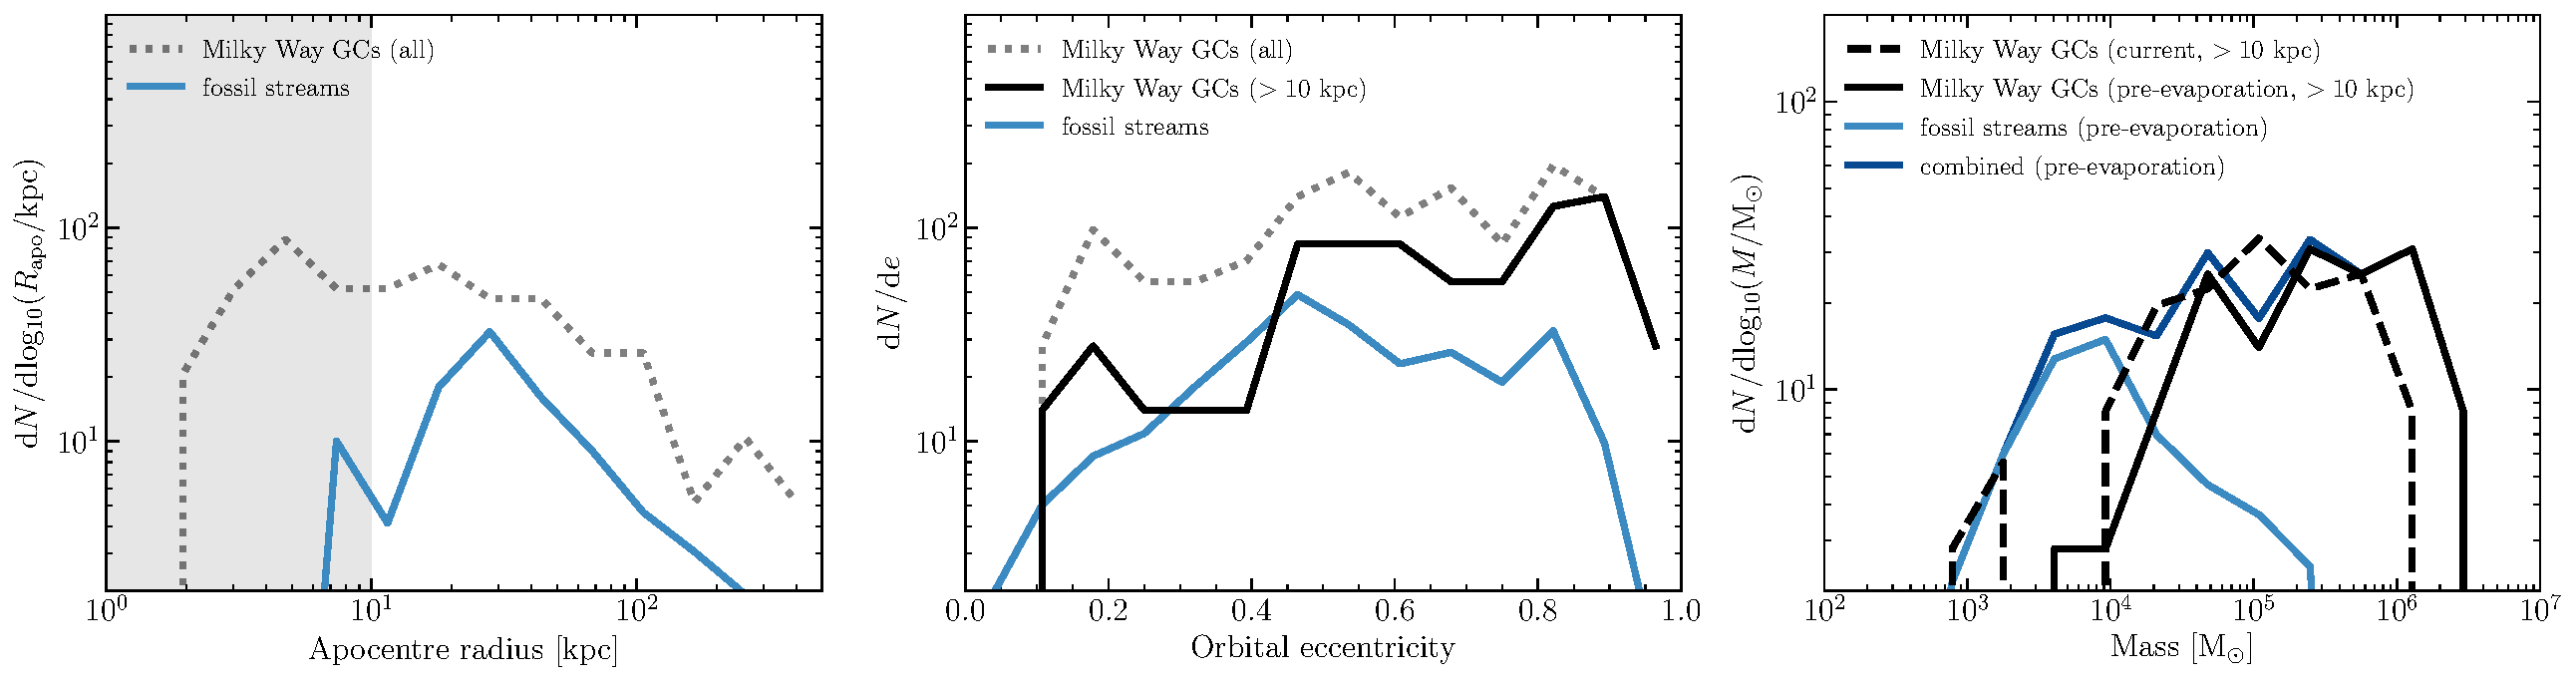
\includegraphics[width=\hsize]{figures/distributions_mc.pdf}%
\caption{
\label{fig:hist}
Demographics of fossil streams (and their progenitor clusters) compared to those of the Galactic globular cluster population. Left: Apocentre radius distributions. The gray-shaded area indicates the inner radii ($\leq10$~kpc) where few fossil streams are found. In the middle and right panels, we therefore consider the globular clusters outside of these radii. Middle: Orbital eccentricity distributions. globular clusters have a weak excess of high eccentricities relative to fossil streams. Right: Mass distributions, both for current globular clusters and for the masses of fossil streams and globular clusters after rewinding their evaporation-driven mass loss in the Galactic halo. The progenitors of fossil streams were systematically a factor of $>10$ less massive than globular clusters.}
\end{figure*}	
We propagate the uncertainties on the fossil streams' orbital parameters into those on the pre-evaporation masses by applying eq.~(\ref{eq:m0}) to the entire sample of MCMC solutions. The resulting distributions of all apocenter radii, eccentricities, and pre-evaporation masses of the fossil streams in the MCMC sample are shown in \autoref{fig:hist}, where we also include the population statistics of Galactic globular clusters that have survived till the present day \citep[2010 edition]{harris96}. For these surviving globular clusters, we also include an estimate of their pre-evaporation masses.

\autoref{fig:hist} reveals interesting differences between the demographics of fossil streams and globular clusters. First, there is a dearth of streams with apocentre radii $\leq10$~kpc. We attribute this to incompleteness, as it is more challenging to identify streams within the solar circle. At larger radii, the streams follow approximately the same apocentre radius distribution as globular clusters. For this reason, we exclude globular clusters with apocentre radii $\leq10$~kpc in the subsequent panels. Second, we find that the eccentricity distribution of streams falls below the distribution of globular clusters at large eccentricities. This result is somewhat counterintuitive, because globular clusters on eccentric orbits are expected to be disrupted more rapidly (see equation~\ref{eq:t0}). Rather than being the result of cluster disruption, we expect the difference in eccentricity distributions to result from the rapid disruption of fossil streams on plunging, eccentric orbits. A strongly decreased lifetime of streams with high eccentricities could naturally produce the observed difference.

Finally, and most interestingly, the pre-evaporation masses of fossil streams and globular clusters differ significantly. The median pre-evaporation mass of fossil streams is just $9\times10^3~\msun$, compared to $5\times10^5~\msun$ for globular clusters (and $1.5\times10^5~\msun$ for the current globular cluster masses). This factor-of-60 difference in pre-evaporation mass directly reflects the fundamentally different nature of both classes of objects. globular clusters must have had the right properties to enable their survival over nearly a Hubble time, whereas fossil streams were disrupted by definition. Since the orbital distributions only show mild differences when limiting the sample to apocentre radii $>10$~kpc, the pre-evaporation mass determines almost entirely whether a cluster survives as a globular cluster or results in a fossil stream.

\begin{figure*}
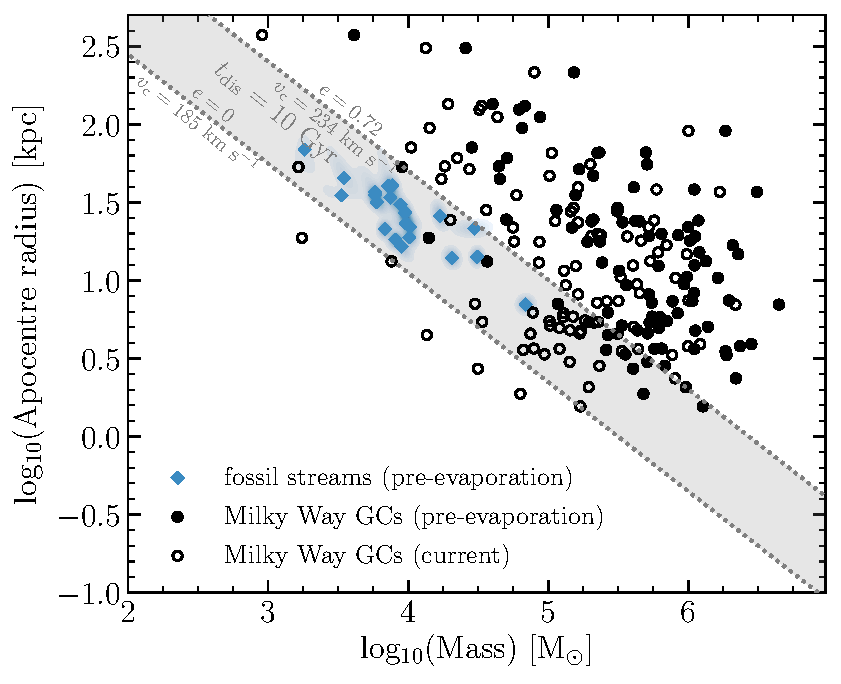
\includegraphics[width=0.5\hsize]{figures/mass_rapo.pdf}\\
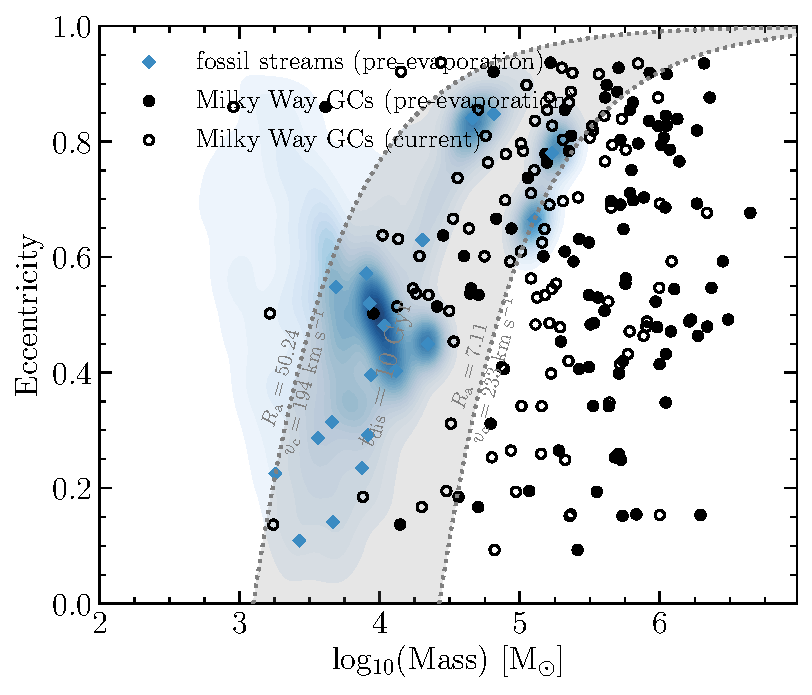
\includegraphics[width=0.5\hsize]{figures/mass_ecc.pdf}%
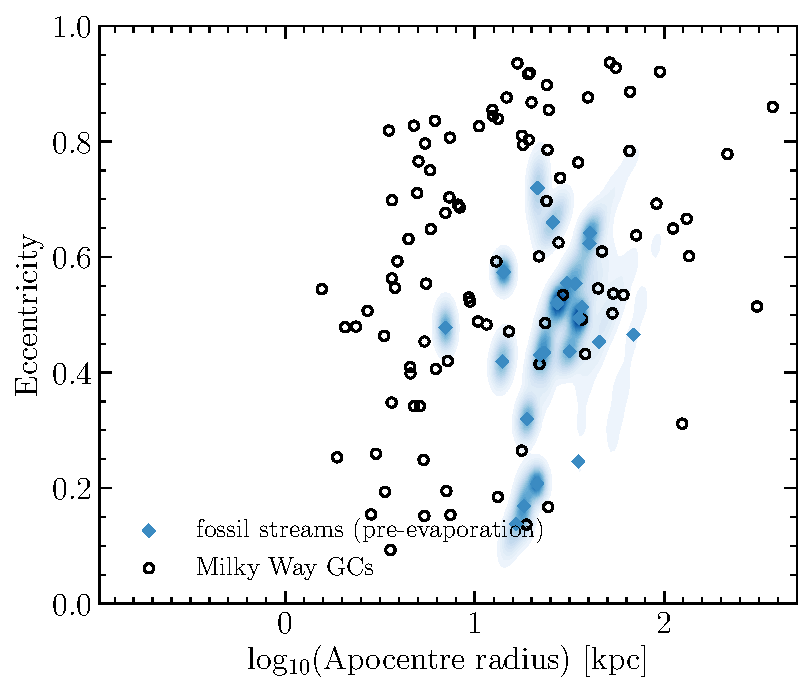
\includegraphics[width=0.5\hsize]{figures/rapo_ecc.pdf}%
\caption{
\label{fig:kde}
Two-dimensional demographics of fossil streams progenitors compared to those of the Galactic globular cluster population. Top left: Mass-apocentre radius plane. Bottom left: Mass-eccentricity plane. Bottom right: Apocentre radius-eccentricity plane. In each panel, the contours show a two-dimensional Gaussian kernel density estimate for the fossil stream progenitors, using the complete sample of MCMC realizations. Blue symbols show the best-fitting result for each fossil stream. Open black symbols show current globular clusters, whereas filled black symbols show their pre-evaporation masses, i.e.\ those corrected for evaporation-driven mass loss on their current orbits. In each panel, the gray-shaded band shows the range in each panel that is predicted to be occupied by the fossil stream progenitors assuming 10~Gyr of evolution, given their range of best-fitting orbital properties and progenitor masses (indicated by the annotations in gray). The fossil stream progenitors are generally clearly offset from the globular clusters.}
\end{figure*}

\autoref{fig:kde} shows the two-dimensional projections of the same quantities as in \autoref{fig:hist}, together with the region within which clusters are predicted to be disrupted within 10~Gyr for the observed stream properties. As expected, the streams fall within this region, which is systematically offset from the distributions of globular clusters, irrespectively of whether we adopt current or pre-evaporation globular cluster masses. Stream progenitors had lower masses (needed to end up as a stream at the present day), have somewhat lower eccentricities (because streams with high eccentricities are disrupted at pericentre), and occupied larger radii (because streams at small radii are difficult to observe and may survive less long). Interestingly, the difference in apocentre radii manifests itself most strongly at low eccentricities. It is well known that the orbits globular clusters become radially anisotropic towards larger radii \citep[e.g.][]{dinescu99}, and the fossil streams do not follow the same behaviour. We expect this difference to be driven by a combination of incompleteness of the stream sample and stream survival. {\color{red}Ana, thoughts?} Finally, the top-left panel of \autoref{fig:kde} shows that the lack of streams with small apocentre radii limits their possible pre-evaporation masses to $<3\times10^5~\msun$. However, this is not responsible for the mass offset that we find. Even when extrapolating the expected distribution of the stream sample to small apocentre radii (along the gray band), the pre-evaporation masses remain about an order of magnitude lower than those of globular clusters.


\section{Discussion}
\label{sec:discussion}

We determined the orbits of 20 globular clusters disrupted in the Milky Way by fitting sky positions, distances, and proper motions of the remnant stellar streams.
Assuming that the progenitor clusters dissolved recently, we integrated the orbit-dependent mass-loss rate to infer their pre-evaporation masses.
Surprisingly, the orbital distribution of disrupted globular clusters, in particular their apocenters and eccentricities, is similar to the orbital properties of the surviving population.
On the other hand, the inferred masses of disrupted globular clusters peak at $10^4\,\msun$---significantly lower than the mass of a typical globular cluster in the Milky Way today.
In this section we discuss this population of low-mass, disrupted globular clusters as tracers of both the Galactic gravitational potential and early star formation, and conclude with an outlook for future follow-up studies.

- implications for individual streams
- compare to mass estimates in the detect part of the stream -> are they mostly detected or are they extending past the currently detected endpoints? -- some were being connected -- is it dynamically plausible
- lower mass -> implications for epicycles: check andreas' paper
- make specific comments for individual streams (e.g., gd-1)
-- if preprocessed, some features might indeed be nature rather than nurture

Most processes that destroy globular clusters operate more efficiently closer to the Galactic center \citep[e.g.,][]{gnedin:1997}.
Hence, if the initial population of globular clusters sampled the orbital space uniformly, we might expect to preferentially find stellar streams on more eccentric orbits with smaller apocenters.
However, streams from our sample occupy similar orbital families as the present-day globular clusters, and the main difference between the two populations is the lower average mass of disrupted clusters.
This may indicate that most globular clusters that ever orbited the Milky Way can be associated with a handful of its progenitor galaxies, in agreement with the phase-space \citep{massari:2019} and age-metallicity \citep{kruijssen19e,kruijssen20} distributions of the surviving cluster population.
Partly, streams with small apocenters and those with high eccentricities may be missing from our sample due to observational biases: low eccentricity tidal debris is more readily identifiable as a thin stellar stream \citep{hendel:2015}, while searching for streams in the inner Galaxy is challenging due to high contamination from the field Milky Way stars \citep[e.g.,][]{ibata:2019}.
The wealth of observational data expected over the next decade will allow for a more complete census of stellar streams that can further test the emerging picture in which the initial population of Galactic globular clusters originates from a small number of host galaxies.

Low-mass clusters are more susceptible to disruption \citep[e.g.,][]{fall:2001}.
As a result, globular clusters, which are predominantly old, peak at a characteristic mass of $\approx10^5\,\msun$ \citep[e.g.,][]{harris:1991}, whereas the masses of young clusters follow a power law distribution \citep[e.g.,][]{zhang:1999}.
As expected for disrupted globular clusters, we find that the masses of stellar stream progenitors are lower than those of still bound clusters.
However, the combined distribution of pre-evaporation masses for stream progenitors and surviving clusters is much shallower than the initial cluster mass function.
In part, the comparative dearth of low-mass clusters may be attributed to incompleteness in the stream sample and the finite lifetimes of the streams, but it may also signify that evaporation is a subdominant cluster disruption mechanism.
For example, \citet{kruijssen15b} proposed that most early-forming clusters were rapidly disrupted in the turbulent disks of their host galaxies, and that only a small fraction of the initial cluster population survives long enough to experience evaporation.
A complete census of stellar streams could therefore inform on dynamical properties of star-forming galaxies at high redshift.

\begin{figure}
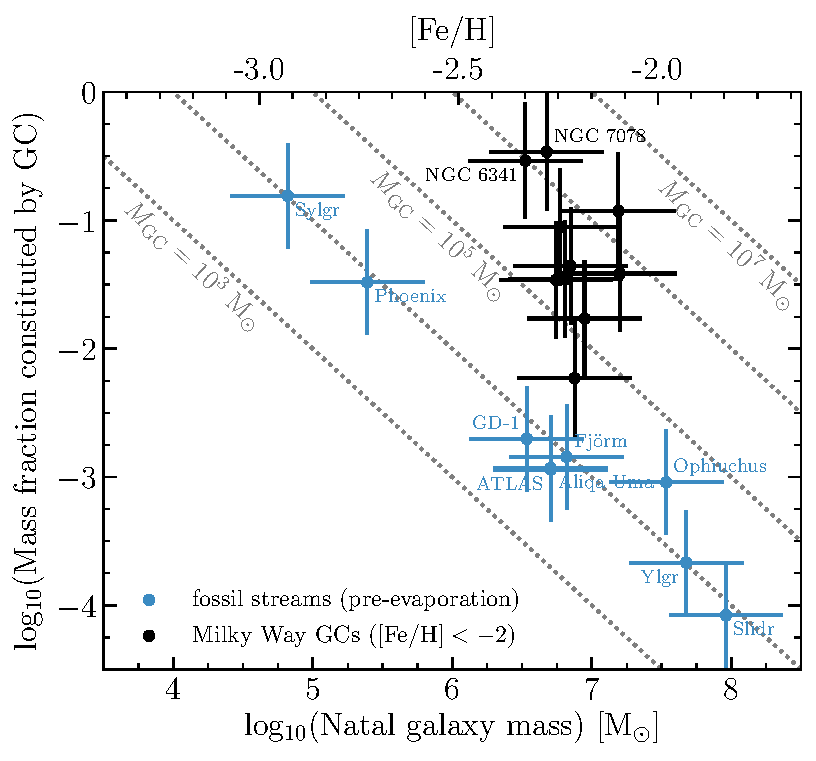
\includegraphics[width=\hsize]{figures/mhost_fraction.pdf}
\caption{
\label{fig:mhost}
Mass fraction of the natal galaxy constituted by the progenitors of fossil streams (blue) and low-metallicity globular clusters (black) as a function of the galaxy mass.
% The sample is restricted to fossil streams with known metallicities, which are converted to a natal galaxy mass using the galaxy mass-metallicity relation between $z=3$ and $z=6$.
Error bars combine metallicity uncertainties with the evolution of the mass-metallicity relation across this redshift range.
On average, stream progenitors constituted a smaller fraction of their natal galaxy's mass than globular clusters, but the progenitors of the most metal-poor streams likely represented a significant fraction of the lowest-mass galaxies ever to exist.
}
\end{figure}

We can place the pre-evaporation masses of the progenitor clusters in the context of their natal galaxy by assuming that at birth they had the same metallicity as their host galaxy, and using the metallicity of the stream to infer the galaxy mass at the time of cluster formation \citep{kruijssen20b}. This is possible, because the galaxy mass-metallicity relation is predicted to exhibit little evolution over the formation redshift range of the metal-poor clusters considered here, such that the stream metallicity mostly traces the natal galaxy mass, rather than the formation redshift. Metallicities are available for seven of the streams in our sample (Aliqa Uma, ATLAS, Fj\"orm, Phoenix, Slidr, Sylgr, and Ylgr; \citealt{ibata:2019,li:2020,wan20}). We follow \citet{kruijssen19c} and convert these metallicities to natal galaxy masses using the galaxy mass-metallicity relation between $z=3$ and $z=6$ predicted by the FIRE simulations \citep{ma16}.

\autoref{fig:mhost} shows the resulting relation between the galaxy mass fraction constituted by the stream progenitor clusters (using their pre-evaporation masses) and the natal galaxy mass. For comparison, we are also including the ten GCs with metallicities $[{\rm Fe}/{\rm H}]<-2$ from the compilation of \citet{kruijssen19e}. The ranges of pre-evaporation masses of streams ($10^{3.5}{-}10^{4.7}~\msun$) and globular clusters ($10^{4.6}{-}10^{6.3}~\msun$) are each considerably narrower than the total range of natal galaxy masses ($10^{4.8}{-}10^{8.0}~\msun$). As a result, the galaxy mass fraction constituted at birth is controlled primarily by the natal galaxy mass, such that the fraction decreases with galaxy mass and metallicity. The typical mass fraction constituted by stream progenitors must have been of the order $10^{-3}$ (due to their low masses), whereas it was typically a few percent for the metal-poor GCs considered here. The two very most metal-poor GCs (NGC~6341 and NGC~7078) may have constituted anywhere between 10--100\% of their host galaxies.

For the streams, the highest fractions are also found at the lowest metallicities. The recently-measured metallicity of the Phoenix stream \citep{wan20} implies that its progenitor cluster represented $2.8_{-1.8}^{+5.3}$\% of its host galaxy at formation, whereas we estimate that the progenitor of the extremely metal-poor Sylgr stream \citep{ibata:2019,roederer:2019} represented $33_{-20}^{+52}$\% of its host galaxy. This is means that the progenitors of fossil streams below the GC `metallicity floor' \citep{beasley19,kruijssen19c} of $[{\rm Fe}/{\rm H}]\approx-2.5$ (or equivalently in galaxies with stellar masses $\la10^6~\msun$) may have represented a relevant fraction of the host galaxy mass, ranging anywhere from 1--100\%. Individual stream progenitors of such high masses may have had a profound impact on the early formation of the host galaxy and potentially its reionization. In future observations of galaxies with stellar masses $\la10^6~\msun$ with the \textit{James Webb Space Telescope}, such progenitor clusters should manifest themselves as bright knots. These systems should not survive as GCs, because they would fall below the GC metallicity floor observed at $z=0$, but they are potential stream progenitors. Such high-redshift observations would directly connect the galactic archaeological results presented in this paper to direct observations of the young stellar systems in their birth environments.

%- what were they in the context of the host galaxy
%- under the assumption that at birth they clusters had the same metallicity as the ambient galaxy, estimate its mass from mass-metallicity relation (cite).
%% The sample is restricted to fossil streams with known metallicities, which are converted to a natal galaxy mass using the galaxy mass-metallicity relation between $z=3$ and $z=6$.
%metallicities available for a subset of streams (cite), shown in blue in figure~\ref{fig:mhost}
%Error bars combine metallicity uncertainties with the evolution of the mass-metallicity relation across this redshift range.
%- as a comparison, low-metallicity globular clusters are shown in black
%- don't expect bound clusters to be dominant mode of sf -- even the more massive gc only contribute 1\% to 30\%
%- the streams have lower mass, so most contribute even less
%- however: some streams lower metallicity, therefore originating from a lower mass galaxy
%- there it dominated the stellar mass budget, and might have had a profound impact on the early formation (keep the galaxy reionized for a while)
%- could be just stochasticity: extending this analysis to more streams will show how common this scenario is
%
%- after fig 4: make prediction for jwst
%- if jwst sees below mstar<~1e6Msun, you see bright knots -- not a surviving gc, but a stream progenitor
%-- explore puny mass range


\vspace{0.5cm}
It is a pleasure to thank: Charlie Conroy.
J.M.D.K.\ gratefully acknowledges the generous hospitality of the Institute for Theory and Computation at Harvard University, where part of this work was carried out. J.M.D.K.\ gratefully acknowledges funding from the Deutsche Forschungsgemeinschaft (DFG, German Research Foundation) through an Emmy Noether Research Group (grant number KR4801/1-1) and the DFG Sachbeihilfe (grant number KR4801/2-1), as well as from the European Research Council (ERC) under the European Union's Horizon 2020 research and innovation programme via the ERC Starting Grant MUSTANG (grant agreement number 714907).

\software{
\package{Astropy} \citep{astropy, astropy:2018},
\package{gala} \citep{gala},
\package{IPython} \citep{ipython},
\package{matplotlib} \citep{mpl},
\package{numpy} \citep{numpy},
\package{scipy} \citep{scipy}
}

\bibliographystyle{aasjournal}
\bibliography{disrupted_gc}


\end{document}


